%! Author = mario
%! Date = 30.01.2023

\section{Game Implementation}\label{sec:game-implementation}

\subsection{Game board}\label{subsec:game-board}
The basic setup of the game is simple, yet the hard parts lie in the way the game is played.
As shown in Fig.~\ref{fig:wooden_board} the game board is made out of wood and tilt-able on two disconnected axes.
This allows the player to move the marble around without direct contact, just by leveraging gravitation.
The goal of this game is to reach the end on the right hand side of the board, without falling into a hole.
If the marble falls down, the player has to restart and is rewarded with the points that are associated with each hole.
To follow the rules, the marble has to pass the holes in the correct order given by the black line.
Only if these requirements are met, the player can win the game.
There is no time limit in this game.\\
The basic concepts are easy to learn, but solving the task is hard to master.
The game requires fine adjustments to the angles and quick reactions to prevent the marble from rolling uncontrolled through
the labyrinth.

\begin{figure}[h]
    \centering
    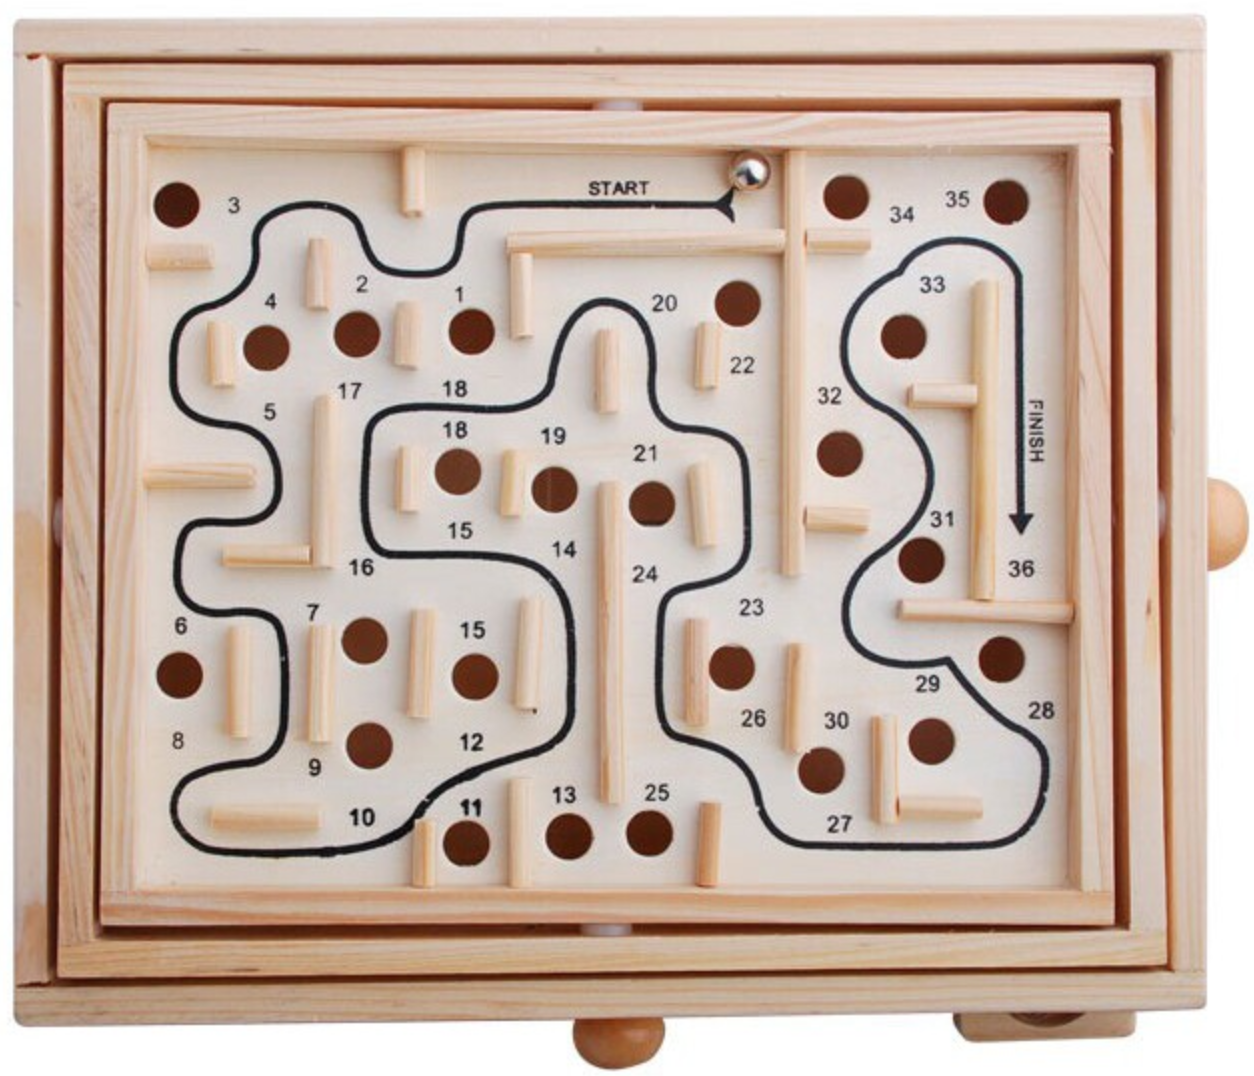
\includegraphics[width=0.65\textwidth]{images/wooden_game_board}
    \caption{The wooden game board, with the path to follow. Source:~\cite{wooden_board}}
    \label{fig:wooden_board}
\end{figure}

\subsection{Unity game board}\label{subsec:unity-game-board}
